\documentclass[
	12pt,
	a4paper,
	BCOR10mm,
	%chapterprefix,
	DIV14,
	listof=totoc,
	bibliography=totoc,
	headsepline
]{scrreprt}

\usepackage[T1]{fontenc}
\usepackage[utf8]{inputenc}
\usepackage{ngerman}

\usepackage{lmodern}

\usepackage[footnote]{acronym}
\usepackage[page,toc]{appendix}
\usepackage{fancyhdr}
\usepackage{float}
\usepackage{graphicx}
\usepackage[pdfborder={0 0 0}]{hyperref}
\usepackage[htt]{hyphenat}
\usepackage{listings}
\usepackage{lscape}
\usepackage{microtype}
\usepackage{nicefrac}
\usepackage{subfig}
\usepackage{textcomp}
\usepackage[subfigure,titles]{tocloft}
\usepackage{units}

\lstset{
	basicstyle=\ttfamily,
	frame=single,
	numbers=left,
	language=C,
	breaklines=true,
	breakatwhitespace=true,
	postbreak=\hbox{$\hookrightarrow$ },
	showstringspaces=false,
	tabsize=4
}

\renewcommand*{\lstlistlistingname}{Listingverzeichnis}

\renewcommand*{\appendixname}{Anhang}
\renewcommand*{\appendixtocname}{Anhänge}
\renewcommand*{\appendixpagename}{Anhänge}

\begin{document}

\begin{titlepage}
	\begin{center}
		{\titlefont\huge Solitaire-Schach\par}

		\bigskip
		\bigskip

		{\titlefont\Large --- Praktikumsbericht ---\par}

		\bigskip
		\bigskip

		{\large Arbeitsbereich Wissenschaftliches Rechnen\\
		Fachbereich Informatik\\
		Fakultät für Mathematik, Informatik und Naturwissenschaften\\
		Universität Hamburg\par}
	\end{center}

	\vfill

	{\large \begin{tabular}{ll}
		Vorgelegt von: & Kira Duwe\\
		E-Mail-Adresse: & \href{mailto:adresse@email.de}{0duwe@informatik.uni-hamburg.de} \\
		Matrikelnummer: & 6225091 \\
		Studiengang: & Informatik \\
		\\
			Vorgelegt von: & Enno Zickler\\
		E-Mail-Adresse: & \href{mailto:adresse@email.de}{0zickler@informatik.uni-hamburg.de} \\
		Matrikelnummer: & 6250134 \\
		Studiengang: & Informatik \\
		\\
		%Erstgutachter: & Name des Erstgutachters \\
		%Zweitgutachter: & Name des Zweitgutachters\\ \\
		Betreuer: & Julian Kunkel \\
		\\
		Hamburg, den 09.10.2013
	\end{tabular}\par}
\end{titlepage}

\chapter*{Abstract}

\thispagestyle{empty}

Solitaire-Schach ist eine Solitairevariante, die ebenfalls allein aber nach Schachregeln gespielt wird. Ziel ist es, dass nur noch eine Figur auf dem Spielbrett übrig bleibt. In jedem Zug muss genau eine Figur geschlagen werden. Die Figuren sind normale Schachfiguren mit ihren üblichen Zugmöglichkeiten. Ausnahme ist nur der Bauer, da er hier in alle Richtungen ziehen kann. Die Startaufstellung auf einem 4x4 Schachbrett besteht aus einer beliebigen Kombination der folgenden Figuren: 1x Dame, 1x König, 2x Springer, 2x Läufer, 2x Turm und 2x Bauer. \\
Unser Programm errechnet, wie viele dieser Startpositionen lösbar sind. Dies ist für Spielbretter bis zur Größe von 21 Feldern (3x7) möglich. Da es für ein 4x4 großes Spielbrett bereits 6,7 Milliarden gültiger Startbelegungen gibt, kann unser Programm auch mit verschiedenen Parallelisierungsstufen auf einem Cluster aufgerufen werden. Parallelisiert wurde mit MPI und OpenMP.

%Inhaltsverzeichnis
\tableofcontents

%Kapitel 1
\chapter{Einleitung}
\label{Einleitung}


\section{Begrifflichkeiten}
Hier eine Definition der im folgenden gebrauchten Begriffe:
\begin{itemize}
	\item Spielbrett: die aktuelle Belegung der einzelnen Felder
	\item Spielfeld: genau ein Einzelsegment des Spielbrettes
	\item Spielbrettbreite: x-Koordinate des Spielbrettes (links-rechts)
	\item Spielbretthöhe: y-Koordinate des Spielbrettes (oben-unten)
	\item Felderanzahl= Spielbrettbreite x Spielbretthöhe
\end{itemize}


\section{Spielregeln}
Solitaireschach ist eine Kombination aus der Spiellogik von Solitaire und 
den Zugregeln des Schachs. Es wird allein auf einem 4x4 großen Brett mit einer gegebenen Startaufstellung gespielt. Diese ergibt sich zufällig aus der Figurenmenge des Schachs, wobei nur zwei Bauern vorhanden sind. Es gibt also eine Dame,
einen König, zwei Springer, zwei Läufer, zwei Türme und zwei Bauern. 
Zu Beginn kann eine beliebige Kombination dieser Figuren auf dem Brett stehen, wobei mindestens zwei und maximal zehn Figuren benutzt werden.
Ungültig wären Spielbretter bei denen zum Beispiel zwei Damen aufgestellt sind.


Ziel ist es, dass am Ende des Spiels nur noch eine einzige Figur auf dem Spielbrett steht. Pro Zug muss genau eine Figur gezogen und damit eine andere geschlagen werden.
Die Figuren ziehen nach folgenden Regeln:
\begin{itemize}
\item Bauer: 
Der Bauer kann auf eines seiner benachbarten Diagonalfelder ziehen. Im Gegensatz zum Schach ist hier jede Zugrichtung möglich.
\item Turm: Der kann beliebig viele Felder (mindestens eines) auf der x- oder auf der y-Koordinate seines Feldes ziehen.
\item Läufer: Der Läufer kann beliebig viele Felder (mindestens eines) auf den Diagonalen seines Feldes ziehen.
\item Springer: Der Springer ist die einzige Figur, die über andere Figuren auf ihrem Weg hinwegspringen kann. Erst die Figur am Ende des Zuges wird geschlagen. Es gibt zwei mögliche Züge. Entweder der Springer wird zwei Felder auf der x-Koordinate und eines auf der y-Koordinate gezogen oder ein Feld in x-Richtung und zwei in y-Richtung. 
\item König: Der König kann genau ein Feld weit ziehen, wobei alle benachbarten Felder möglich sind. Er stellt also eine Mischung aus Bauer und eingeschränktem Turm dar.
\item Dame: Die Dame ist in der Lage beliebig viele Felder auf den Diagnoalen oder auf einer der beiden Achsen zu ziehen. Damit ist sie eine Kombination aus Läufer und Turm.
\end{itemize}


\section{Aufgabenstellung}

Das Spiel bietet nun eine enorme Vielfalt an gültigen Startpositionen und resultierenden Folgebrettern.
Uns faszinierte daher die Frage, wie viele mögliche Startbelegungen es gäbe und welche davon lösbar wären.
Dieses Problem wollten wir gern für eine variable Spielbrettgröße untersuchen und nicht nur für den Fall des 4x4-Brettes.
Das Programm sollte also alle gültigen Startpositionen erzeugen - und zwar nur die gültigen - sowie eine Berechnung durchführen, welche dieser entstandenen Bretter lösbar sind.
Sollten diese Aufgabenstellungen nicht umfangreich genug sein, so hätten wir uns noch mit der Ausgabe der möglichen Lösungen beschäftigt und einer Aufzeichnung der Lösungswege.
Gegen die Ausgabe der verschiedenen Lösungswege entschieden wir uns, da der Bedarf an Speicherplatz jeglichen Rahmen gesprengt hätte.


%Kapitel 2
\chapter{Entwurf \& Implementierung}
\label{Entwurf}

\section{Entwurf}
\section{Probleme}
Während des Entwurfs und der Implementierung traten in einigen Bereichen Schwierigkeiten auf.
\subsection{Spielbretterzeugung}
Zunächst einmal bestand der Anspruch nicht nur einen korrekten sondern auch einen effizienten Algorithmus für die Erzeugung der Spielbretter auf einer variablen Spielbrettgröße zu finden.
Es sollten also garantiert alle Spielbretter erzeugt werden, ohne dass doppelte entstehen.

\subsection{Modellierung und Speicherung der Spielbretter}
Eine obere Grenze für die Anzahl der möglichen Startbelegungen bietet eine Abschätzung mit der Faktoriellen:\\
16 * 15 * 14 * 13 * 12 * 11 * 10 * 9 * 8 * 7 = 29 059 430 400

Dort sind zwar noch die doppelten Felder enthalten, die dadurch entstehen, dass zwischen den Figuren vom gleichen Typ nicht unterschieden wird, dennoch bietet es eine gute Einschätzung der Größenordnung.
Damit ergab sich die Frage, wie man die Spielbretter möglichst speichereffizient modellieren kann und wie eine sinnvolle Speicherverwaltung einer derart großen Menge aussehen könnte, die später auch noch für den parallelen Zugriff geeignet wäre.

\subsection{Berechnung der Spielbretter}
Um von einer gültigen Startbelegung zu der Aussage  "`Das Brett ist lösbar."' zu kommen,braucht man mindestens einen im Maximalfall aber 9 Berechnungsschritte und zwar für jedes Spielbrett. Da die Zahl der möglichen Spielbretter ohnehin schon sehr groß ist, musste also eine Berechnung gefunden werden, die sehr effizient arbeitet.


\subsection{Lastungleichheit}
Aufgrund der Abhängigkeit der Berechnungszeit von der Anzahl der möglichen Züge ergibt sich eine deutliche Lastungleichheit. Es lässt sich nicht sagen, wie viele Figuren überprüft werden müssen, bis ein als lösbares gespeichertes Nachfolgebrett entsteht. 



\section{Implementierung}
\subsection{Darstellung der Spielbretter}
Wir schwankten lange zwischen zwei verschiedenen Ansätzen.
Eine Möglichkeit ist die Speicherung als zweidimensionales Array, das eine deutlich intuitivere Handhabung mit sich bringt. Allerdings ist es deutlich größer, was den benötigten Speicher angeht.
Das kleinste zur Verfügung stehende wäre ein 16 elementiges Char-Array. 
Es braucht also für den Fall 4x4:  16*8bit = 128 bit.

Um eine möglichst kompakte und damit speicher- und zugriffseffiziente Darstellung der Spielbretter zu erhalten, entschieden wir uns für eine Oktaldarstellung. Diese benötigt 64 bit und bietet die Möglichkeit, Spielbretter bis zu einer Größe von 3 x 7 zu codieren. 
Das 4x4 Brett braucht also nur 64 bit und damit die Hälfte im Vergleich zum Array.

Codierung:\\
Die letzte Stelle der Zahl ist das Feld des Brettes mit der Nummer 0.
Jede Stelle der Oktalzahl bzw. drei Stellen der Binärzahl ($ 2^3 = 8 $) repräsentiert also genau ein Feld des Spielbrettes. Für die Spielfiguren führten wir folgende Codierung ein:
\begin{itemize}
\item 0 = leeres Feld
\item 1 = Bauer
\item 2 = Turm
\item 3 = Läufer
\item 4 = Springer
\item 5 = König
\item 6 = Dame
\end{itemize}

Die Felder des Spielbrettes nummerierten wir von 0 - Felderanzahl-1 durch.
\begin{table}
	\begin{center}
		\begin{tabular}{|c|c|c|c|}\hline
		 0 &  1 &  2 &  3 \\ \hline
		 4 &  5 &  6 &  7 \\ \hline
		 8 &  9 & 10 & 11 \\ \hline
		12 & 13 & 14 & 15  \\ \hline
		\end{tabular}
	\end{center}
	\caption{Nummerierung der Spielfelder}
	\label{table:Tabelle1}
\end{table}

Hier ein Beispiel wie für die Darstellung eines Spielbrettes als Oktalzahl.
Das Spielbrett:  3032 4124 0650 0010 entspricht dem in der Tabelle dargestellten.
\begin{table}
	\begin{center}
		\begin{tabular}{|c|c|c|c|}\hline
		 0 &  1 &  0 &  0 \\ \hline
		 0 &  5 &  6 &  0 \\ \hline
		 4 &  2 &  1 & 4 \\ \hline
		 2 &  3 &  0 &  3 \\ \hline
		\end{tabular}
	\end{center}
	\caption{Spielbrett 3032 4124 0650 0010}
	\label{table:Tabelle1}
\end{table} 

Diese Art der Repräsentation orientiert sich an dem gängigen Standard für die Speicherung von Schachbrettern. Dort wird eine Binärzahl mit der Größe von  64 bit benutzt, um darstzustellen, welche Felder belegt sind.
Zwei weitere werden benötigt, um die Figurentypen zu speichern.
Da wir aber ein deutlich kleineres Spielbrett betrachten, entschieden wir uns dafür nur eine Zahl zu benutzen.



\subsection{Erzeugung der Spielbretter}

Die Erzeugung erfolgt über ineinander verschachtelte for-Schleifen.
Der naive Ansatz zählt für jede Figur jeweils von 0 bis Spielbrettgröße.
Da aber zwischen den doppelten Figuren (Springer, Läufer, Turm, Bauer) nicht unterschieden wird, ist es möglich an dieser Stelle zu optimieren.
So beginnt die jeweils zweite Figur die for-Schleifen erst ab der Position der jeweils ersten Figur zu durchlaufen, da ansonsten ein bereits erzeugtes Spielbrett erneut durchlaufen würde.
Eine weitere Optimierung ist möglich, indem alle weiter innen liegenden Schleifendurchläufe abgeschnitten werden, sobald das betrachtete Feld nicht frei ist. Denn es wird unabhängig vom Typ der Figur niemals möglich sein, diese auf ein bereits belegtes Feld zu setzen.

\begin{lstlisting}[caption={Erzeugung der Spielbretter}, label={lst:example1}]
for(2 bis maximaleFigurenanzahl){
//Schleife Dame
for(posDame = 0; posDame <= anzahlFelder; posDame++){	
	if(positionDame<anzahlFelder){
         setze Dame;
         anzahlFiguren ++;
    }
    
    //Schleife Koenig
    for(posKoenig = 0; posKoenig <= anzFelder; posKoenig++){	
    	 // uebernehmen der bisher gesetzen Figuren
         spielbrettKoenig = spielbrettDame;
         // uebernehmen der bisherigen Figurenanzahl
         anzFigurenK = anzFigurenD;
                    
         if(!(anzFigurenK < maxFiguren)){
             setze keinen Koenig;
         }
                                        
         if(feldFrei(posKoenig, spielbrettKoenig)){
              if(posKoenig<anzFelder){
                   setze Koenig;
                   anzahlFiguren ++;
              }
              
              //Schleife 1. Springer 	
              for(posSpringer1 <= anzFelder){
              		...
              		if(!(anzFigurenS < maxFiguren))
              		...
              		if(feldFrei){
              			if(posSpringer < anzFelder)
              			...
              			posSpringer2=posSpringer1;
              			//Schleife 2. Springer
              			for( posSpringer2<=anzFelder){
              			...
              		 	 //Schleifen 1.+ 2. Laeufer
           			 	 ...
       				 	 //Schleifen 1. + 2. Turm
           			 	 ...
              		 	 //Schleife 1. Bauer
       				 	 ... 
              			 //Schleife 2. Bauer
              			 for(Bauer2) {
              				if(! <)
              				if(feldFrei){
		      					 if(<){ 
		      				 	 	setze Bauer2;
		      				 	 	berechneSpielbrett;
              					}
              				}
              			}
              		}
            	}
        	}
    	}
	}
}
\end{lstlisting}

Die äußere for-Schleife sorgt dafür, dass erst alle Spielbretter mit zwei Figuren erzeugt werden und danach aufsteigend alle mit mehr Figuren. Dies ist notwendig, da die Berechnung auf der aufsteigenenden Figurenanzahl aufbaut und in der innersten Schleife direkt aufgerufen wird. Das ermöglicht die Verwendung eines Sets zur Speicherung. (siehe Unterkapitel Speicherung der Spielbretter)
 

\subsection{Berechnung der Spielbretter}
Um die bereits berechneten Lösungen weiter zu verwenden, findet die Berechnung in Abhängigkeit der auf dem Brett befindlichen Figurenanzahl statt.
Zunächst werden alle Bretter mit einer Figur als lösbar vermerkt.
Es findet nun eine ebenenweise Berechnung statt, bei der nach der Figurenanzahl aufgestiegen wird. So kann für jedes Spielbrett einer höheren Ebene überprüft werden, ob daraus ein lösbares Brett entstehen kann. Der Ansatz der dynamischen Programmierung ist eine erhebliche Optimierung, da ohne diese Wiederverwendung im schlechtesten Fall noch acht weitere Berechnungen stattfinden müssten. 

Für die Berechnung werden die Spielbretter nicht nur in der Oktaldarstellung sondern auch als Array vorgehalten. 
Das hat den Vorteil, dass die Abfragen zur Überprüfung ob, eine Spielfigur sich nach einem Zug auch noch auf dem Spielbrett befindet, sehr viel übersichtlicher und verständlicher werden. 
Denn eine für verschiedene Spielbrettgrößen passende Abfrage ist auf Oktalzahlen zu aufwändig.

Es findet also zunächst eine Umwandlung in die Arraydarstellung statt.
(siehe Listing~\ref{lst:example1})
\begin{lstlisting}[caption={Umwandlung in Arraydarstellung}, label={lst:example1}]  
// Berechnung der Arraydarstellung aus Oktaldarstellung einfacher fuer die 
// Ueberpruefung der Spielbrettgrenzen*/
for(x=0; x < SpielbrettBreite; x++)
{
    for(y=0; y < SpielbrettHoehe; y++)
    {   
		param.spielbrett_array[x][y] = 
		(spielbrett >> ((x+(y*SpielbrettBreite)) * 3)) % 8;
        }
    }
\end{lstlisting}

Das daraus entstandene zweidimensionale Array wird nun also Feld für Feld überprüft, ob dort eine Figur steht. Ist dies der Fall wird berechnet, ob es für diese Figur mögliche Züge gibt, die zu einem lösbaren Brett führen.
(siehe Listing~\ref{lst:example2})

\newpage

\begin{lstlisting}[caption={Berechnung eines Spielbrettes}, label={lst:example2}]
 for(x=0; (x < SpielbrettBreite) && (loesbar == 0); x++)
 {
     for(y=0; (y < SpielbrettHoehe) && (loesbar == 0); y++)
	 {   
		switch(param.spielbrett_array[x][y]){
			case DarstellungBauer:
				loesbar= berechneBauer(&param, x, y);
				break;
			case DarstellungTurm:
				loesbar = berechneTurm(&param, x, y);
				break;
			case DarstellungSpringer(&param, x, y);
				break;
			case DarstellungKoenig:
				loesbar = berechneKoenig(&param, x, y);
				break;
			case DarstellungDame:
				loesbar = berechneDame(&param, x, y);
				break;
		}
	}
 }
\end{lstlisting}


Das Schlagen einer Figur geschieht auf der Darstellung als Oktalzahl.
Um die schlagende und die geschlagene Figur vom Brett zu löschen, wird die Oktalzahl mit einer Bitmaske aus Einsen verundet, die an den beiden entsprechenden Positionen eine 0 hat.
Anschließend wird die Figur an die neue Position geschrieben. 


(siehe Listing~\ref{lst:example3})
\begin{lstlisting}[caption={Schlagen einer Figur}, label={lst:example3}]
void schlageFigur()
{
einser_Bitmaske = 0xffffffffffffffffLL;

// Spielfiguren von Spielbrett loeschen 
// Von der Bitmaske wird "(7 << pos*3)" abgezogen, um an dieser Stelle 0 zu erzeugen 
	neues_spielbrett = spielbrett & 
	(einser_Bitmaske - (7 << pos*3) - (7 << neue_pos*3));
	
	// nach Schlagen Spielfigur neu  setzen 
	neues_spielbrett += (DarstellungFigur << neue_pos*3);
}
\end{lstlisting}


\subsection{Speicherung der Spielbretter}

Die ursprüngliche Speicherung der Spielbretter erfolgte nach der Figurenanzahl in verschiedenen Hashtabellen.
In diesen wurde hinterlegt, ob ein Spielbrett lösbar ist (1) oder nicht (0). Verwendet wurde hier ein directhash, da die Spielbrettrepräsentation bereits eindeutig ist.
Aufgrund der enorm großen Anzahl an gültigen Spielbrettern ist das Speichern all dieser 64bit-Integer aber nicht ohne weiteres möglich.

Also optimierten wir die Speicherung. Der nächste Schritt war die Verwendung der Hashtabelle als Set.  
Es wurden also nur noch die lösbaren Bretter gespeichert. Damit entfiel die Speicherung des Wertes, der aufgrund der Signaturen der verwendeten Bibliothek (glib) ebenfalls 64 bit groß gewesen wäre, obwohl wir nur ein Bit benötigt hätten.
Dies war jedoch erst dadurch möglich, dass wir die Erzeugung umbauten, sodass sie die Spielbretter mit zwei Figuren zuerst erzeugte und direkt in der innersten Schleife die Berechnung stattfand.

Im Laufe der Analyse stellte sich heraus, dass die Menge an lösbaren Bretter deutlich größer ist als die Menge der nicht lösbaren. Es gibt sogar Figurenanzahlen, bei denen alle Spielbretter lösbar sind(siehe Kapitel~\ref{Ergebnisse}).
Daher wird die Hashtabelle inzwischen als Set für die Speicherung der nicht lösbaren Spielbretter verwendet.\\
\\
Anzahl lösbare Bretter bei 4x4: 6.683.363.975\\
Anzahl nicht lösbare Bretter bei 4x4: 1.047.721\\

Anfangs war folgender Speicherbedarf notwendig für ein 4x4-Spielbrett:\\
6.684.411.696 x 64bit x 2 = 855.604.697.088 bit = 106 GByte \\
Inzwischen sind es aber nur noch: \\
1.047.721 x 64 bit = 67.054.144 bit = 8,3 MByte\\
\\ 
Eine weitere Optimierung hat dadurch stattgefunden, dass nur noch die aktuellen Bretter und die aus der vorherigen Ebene gespeichert werden und der Rest verworfen wird. Denn für die Berechnung ist jeweils nur das aktuelle Brett und die Information, welche Bretter bisher lösbar waren, notwendig.

\subsection{Parallelisierung}
Für die Parallelisierung haben wir sowohl MPI als auch OpenMP verwendet. Beides lies sich sehr gut auf unsere verschachtelten for-Schleifen anwenden. Wir haben die äußerste Schleife (die der Dame) für die MPI Aufteilung verwendet. Damit ergibt sich hier als Grad der maximalen Parallelität die Anzahl der Felder + 1. Dies reichte für unseren Cluster jedoch vollkommen, da wir für ein 4x4 und sogar für 3x3 Bretter alle 10 Knoten benutzen konnten. 
Um aber auch alle Kerne auf den Knoten zu benutzen, haben wir die nächsten beiden Schleifen mit OpenMP parallelisiert. Umgesetzt wurde dies mit der nested Funktion von OpenMP. Die Benutzung des collapse-Befehls war aufgrund der Abbruchbedingung, ob das Feld schon belegt ist, nicht möglich.


\subsection{Kommunikation}
Der eigentlich Knackpunkt war nach der Aufteilung auf die Knoten die Kommunikation zwischen ihnen. Erst die Speicherplatzoptimierung und vorallem die Möglichkeit, die Spielbretter in der Reihenfolge der Anzahl ihrer Spielfiguren zu erzeugen, machte uns eine eine effiziente Kommunikation möglich.
Wenn wir alle Spielbretter hätten vorhalten müssen, dann wäre es uns nicht möglich gewesen, jedem Knoten auf seinem Speicherplatz alle Spielbretter zur Verfügung zu stellen. Somit hätte es bei jedem Nachgucken, ob ein Spielbrett lösbar ist, zu einer Kommunikation kommen können und in vielen Fällen sogar müssen, da dieser Teil der Daten auf einem anderen Knoten liegt. Durch die Minimierung des Speicherbedarf war es uns jedoch möglich, nach der Berechnung für eine Figurenanzahl die Daten aus dem letzten Berechnungsdurchlauf von jedem Knoten an jeden anderen zu senden, sodass für den nächsten Durchlauf jeder Prozess auf alle vorherigen Ergebnisse zurückgreifen kann.  \\
Hierzu war es nötig, dass alle Prozesse nach einem Durchlauf zunächst über eine MPI-Barrier synchronisiert werden. Anschließend musste jeder Prozess den anderen mitteilen, wie viele Spielbretter er im letzen Durchlauf als nicht lösbar gespeichert hat und den anderen senden möchte. Daraufhin wird in jedem Prozess ein Buffer für die erwarten Spielbretter alloziert. Außerdem muss der Inhalt des eigenen Hashsets in ein Buffer zum Senden kopiert werden.
Zusätzlich werden noch die Zähler für die Anzahl der errechneten Spielbretter vom Master-Prozess eingesammelt, um sie am Ende ausgeben zu können.\\
\\
\\
 
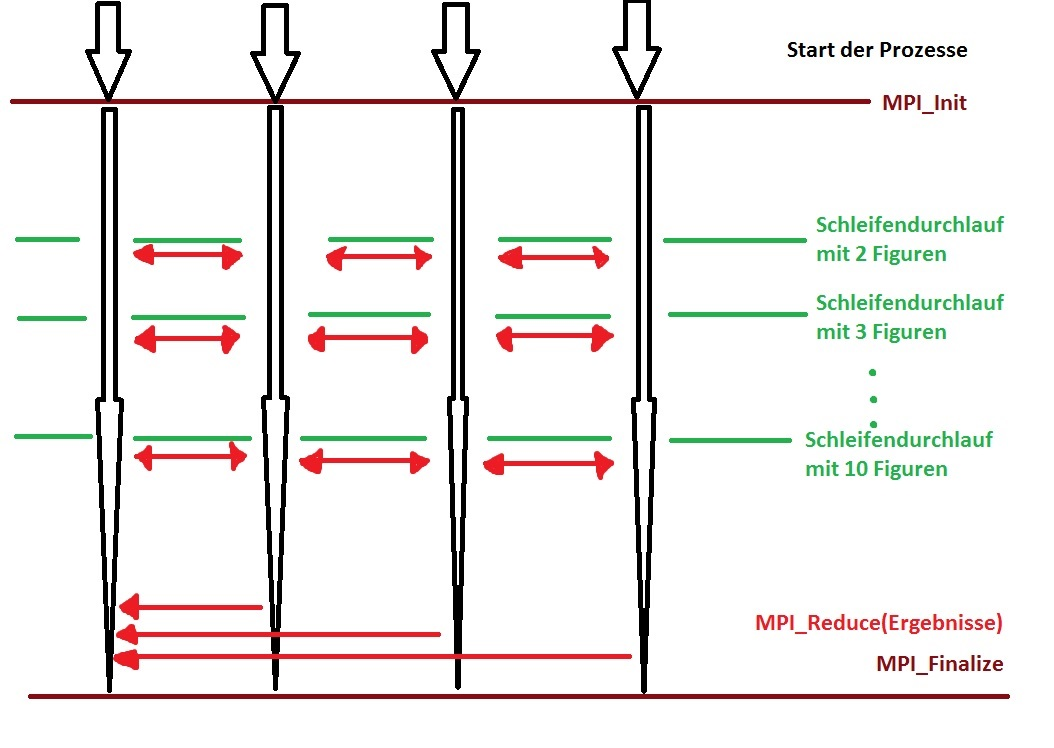
\includegraphics[scale=0.5]{MPI_Kommunikation}


%Kapitel 3
\chapter{Ergebnisse}
\label{Ergebnisse}

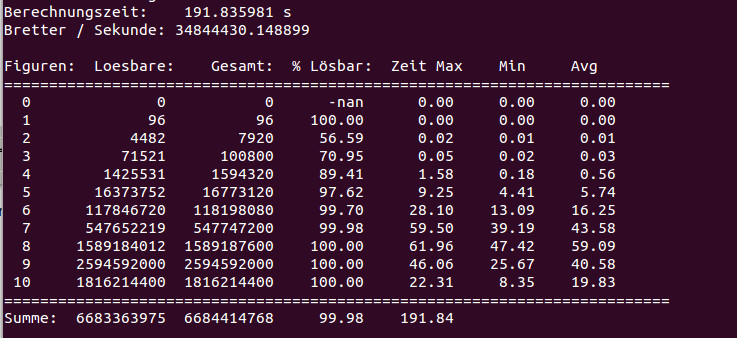
\includegraphics[scale=0.6]{output}
\newline
\newline
Anzahl der gültigen Spielbretter für ein 4x4-Brett = 6.684.411.696 :\\
Anzahl nicht lösbare Bretter bei 4x4: 1.047.721\\

Der Anteil an nicht lösbaren Spielbrettern wird bei größerer Spielbrettgröße immer kleiner. Das hängt damit zusammen, ob eine Dame auf dem Brett platziert ist oder nicht. Je mehr Figuren auf dem Brett stehen, umso größer ist die Wahrscheinlichkeit, dass sich auch die Dame dort befindet. Und die Wahrscheinlichkeit, dass ein Brett lösbar ist, wächst mit der Zahl der aufgestellten Figuren, wenn auch eine Dame gesetzt ist. 
Das liegt an der großen Vielfalt an möglichen Zügen, die eine Dame hat.
So sind die Spielbretter mit zehn Figuren in der Größe 4x4 immer lösbar.

Wir können an dieser Stelle keinen formalen Beweis für die Korrektheit der Behauptung anführen, da jedoch die Menge der nicht lösbaren Bretter gleich blieb, unabhänig davon ob diejenigen mit zehn Figuren mitbetrachtet wurden oder nicht, brauchen diese also nicht mehr berechnet werden. 


\section{Analyse}
Im Profiling des Programms kann man sehr schön sehen, auf welchen Funktionen unsere Berechnung sich am stärksten stützt. Diese sind vorallem die Abfrage bei der Erzeugung, ob ein Feld frei ist und in der Berechnung die Funktion zum Schlagen einer Figur. 
Bei diesen beiden Funktionen haben wir deshalb eine möglichst effiziente Implementierung gewählt. Es zeigt sich aber auch, dass das Umrechnen in ein Array viel Zeit kostet und man hier für weitere Optimierungen doch noch einmal versuchen könnte, die Berechnung vollständig auf den Oktalzahlen zu implementieren.
\\
Gprof des sequentiellen Programms:\\
\\
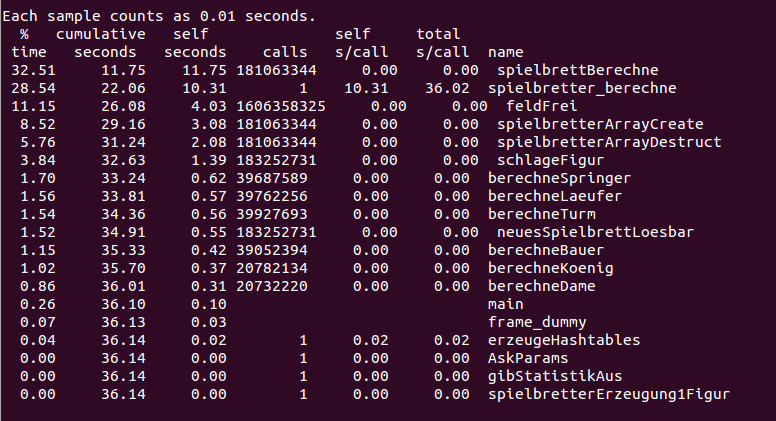
\includegraphics[scale=0.6]{gprof}
\newline
\newline
\newline
Profiling von vampiretrace des parallelen Programms:\\
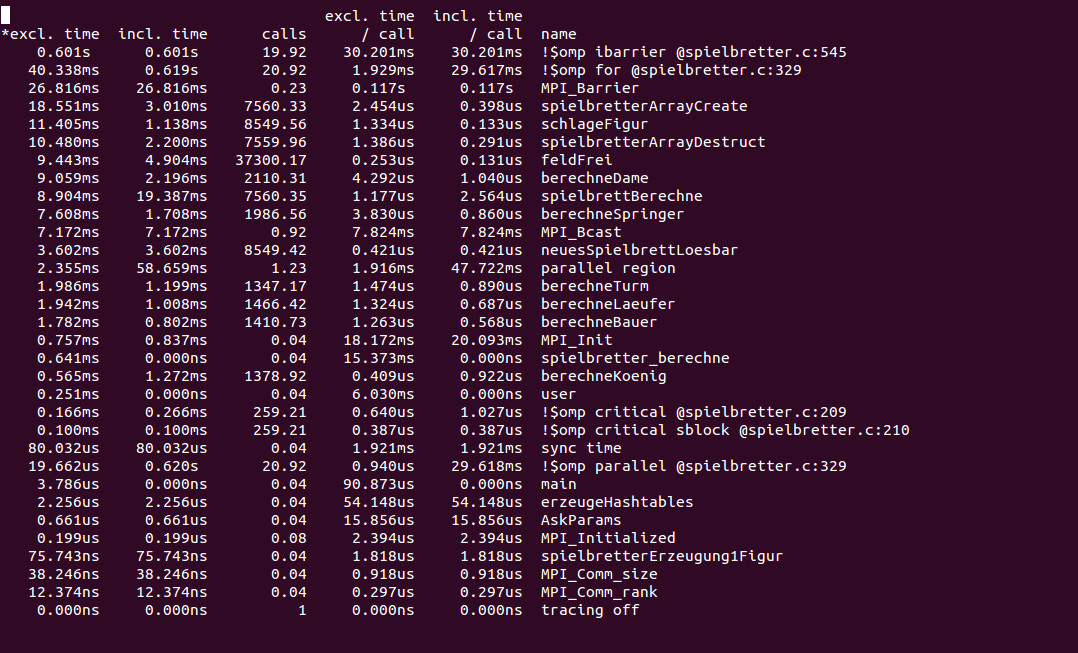
\includegraphics[scale=0.4]{vampirtrace-prof}

Im Profiling der parallelisierten Variante ist auch zu sehen, dass eine gewisse Lastungleichheit eine Menge Zeit kostet. Hierbei scheint die Aufteilung bei OMP jedoch noch schlechter zu sein als bei MPI. Schön ist allerdings, dass der parallele Zugriff auf die glib  Hashtabelle, die eine kritischen Abschnitt für OpenMP darstellt, nicht so sehr ins Gewicht fällt. Dies war insbesondere bei den ersten sequentiellen Programmen ein ganz großes Problem.
\newline

Sehr erfreulich finden wir auch unsere Ergebnisse hinsichtlich Laufzeit, Speicherbedarf und Skalierbarkeit. Wie zuvor schon erwähnt, haben wir die Laufzeit von unserem naivem Ansatz mit einer geschätzten Laufzeit von 17 Tagen auf eine Laufzeit von 93 min und in der parallelen Variant auf 191 sec reduziert. Auch bei dem Speicherbedarf sind wir von erwarteten 106 GByte auf eine Speicherbedarf von unter 10 MByte gekommen. 
Und auch die Skalierbarkeit kann sich durchaus sehen lassen. Ihre Grenzen sind zwar abhängig von der Spielbrettgröße, es ist jedoch auch fraglich, ob sich ein weiterer Performancegewinn noch erzielen ließe, solange kleine und auch große Spielbretter betrachtet werden. Denn auf beispielsweise einem 2x3 Spielbrett würde die Kommunikation einen erheblichen größeren Anteil ausmachen als die eigentliche Berechnung. Damit bringt eine schlichte Erhöhung der Knotenanzahl und Threadanzahl vermutlich kaum noch Nutzen.

\section{Speedup}

In den ersten beiden Diagrammen läst sich gut erkennen, dass der Speedup durch MPI sehr gut ist, aber mit zunehmender Prozessanzahl der Kommunikationsaufwand steigt und sich der Speedup weiter vom Optiumum entfernt. Hinzu kommt sicher auch die nicht ganz optimale Lastverteilung.
Der Speedup durch OpenMP ist hingegen nicht ganz so gut wie bie MPI. Dies wird an der Lastungleichheit und an dem gemeinseam Zugriff auf die Hashtabellen liegen. Trotzdem haben wir auch hiermit ein deutlichen Performancegewinn erzielt.\\

\pagebreak
Speedup mit MPI: 

\includegraphics[scale=0.9]{Laufzeitanalyse24t}

\includegraphics[scale=0.9]{Laufzeitanalyse12t}

\pagebreak
Speedup mit OpenMP:

\includegraphics[scale=0.9]{bretterprosec}

\includegraphics[scale=0.9]{Laufzeitanalyseanzahlthreads}




%Kapitel 4
\chapter{Fazit}
\label{Fazit}


Das Praktikum hat wie kaum eine andere Veranstaltung gezeigt, worauf es bei der praktischen Lösung eines Problems ankommt.

Wir haben Fehler gemacht, wie zum Beispiel "`einfach drauf los"' zu programmieren und erst nach und nach ein Konzept für das Programm zu entwickeln. Dadurch dass wir zu Beginn keine konkrete Vorstellung hatten, wo wir eigentlich hinwollten, war es schwierig einen passenden Zeitplan zu erstellen. 
Inzwischen sind wir also um viele sehr wertvolle Erfahrungen reicher und wissen, wie man bei Null anfangen sollte. 
Zum ersten Mal im Studium sollten wir ein selbst gewähltes Problem modellieren und auch lösen.
Unsere Problemwahl haben wir nie bereut, denn Solitaire-Schach bietet viele Möglichkeiten, um sich als Informatiker damit auseinander zu setzen und hat uns sehr gefesselt.
Die Entwicklung eines Algorithmus, der alle gültigen Startbretter erstellt und zwar nur diese, war ein sehr faszinierender und auch anspruchsvoller Prozess. Sie erforderte zu Beginn einiges an Abstraktionsvermögen, um mit der gewählten Oktaldarstellung erfolgreich arbeiten zu können.
Auch die Notwendigkeit für Optimierungen forderte uns heraus. Zunächst zeichnete sich für das sequentielle Programm eine Laufzeit von 17 Tagen für ein 4x4-Spielbrett ab. 
Diese haben wir inzwischen auf ungefähr eineinhalb Stunden reduzieren können. 
Wir haben also die Aufgabenstellung erfüllt, die wir uns selbst gestellt haben und sind zufrieden mit unseren Ergebnissen.
Unsere Kenntnisse in der C-Programmierung sind erheblich größer und detaillierter, als sie es zu Beginn waren. Gleiches gilt für die Parallelisierung mit MPI und OpenMP.
Die Arbeit auf dem Cluster war sehr lerreich und auch über Jobskripte wissen wir nun einiges mehr. Schlussendlich war es sehr hilfreich mit git zu arbeiten.

Kaum eine andere Veranstaltung war so anspruchsvoll und fordernd und zeitgleich so unglaublich spannend wie das Praktikum.
Die kompetente und freundliche Betreuung hat es zu einem tollen Projekt gemacht.

Einzig der späte Beginn mit der praktischen Umsetzung des eigenen Aufgabe war schade, denn wir hätten gern noch den anderen Lösungsansatz für unser Problem gebaut.
Durch die knappe Zeit am Ende haben wir den mit Julian Kunkel entwickelten "`Bottum-up-Ansatz"' aber leider nicht weiter verfolgen können, sonst wäre für jegliche Analyse keine Zeit mehr geblieben.
 


\end{document}
